\documentclass{hw_template}

\usepackage{arydshln}

\title{\bfseries Лабораторна Робота: Дослідження Кінематики Верхньої 
Кінцівки Людини}
\author{\bfseries Захаров Дмитро}
\date{1 грудня, 2024}

\begin{document}

\pagestyle{fancy}

\maketitle

\section{Умова}
\begin{problems}
    Провести вимірювання і заповнити таблиці. 

    \textbf{Замітка.} 
    
    \begin{itemize}
        \item $AB$ --- довжина сегмента верхньої кінцівки від плечового суглоба (найточніша
    точка кульового суглоба плеча) до ліктьового (виступає кісточки збоку від
    ліктьового суглоба) при зігнутій в лікті руці.
        \item $BC$ --- довжина сегмента верхньої кінцівки від ліктьового суглоба до
    променево‐зап'ясткового (складки між передпліччям і долонею).
        \item $CD_1,\dots,CD_5$ --- довжини сегментів пальців рук від зап'ястя до
    кінчиків пальців.
    \end{itemize}

    \begin{center}
        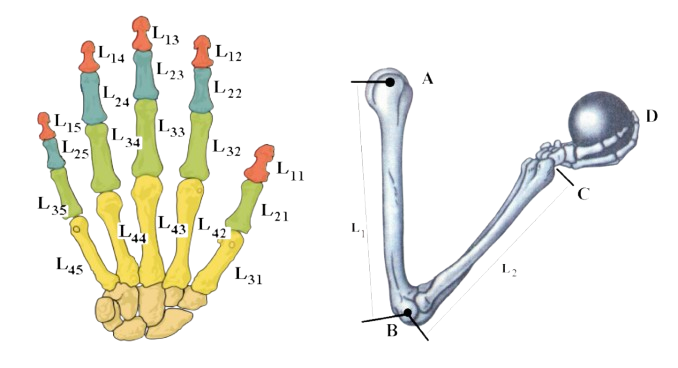
\includegraphics[width=0.8\textwidth]{images/problem_statement.png}

        \scriptsize
        \textbf{Рис.} Позначення з таблиці.
    \end{center}
\end{problems}

\vspace{20px}

\begin{center}
    \large
    \textbf{Дивись таблиці на наступних сторінках.}

    $\to$
\end{center}

\newpage

\section{Параметри верхньої кінцівки}

Міряємо довжини стандартною лінійкою, що вимірює з точністю до $1\,\text{mm}$ ($0.1\,\text{cm}$). Хоч в такому 
випадку прийнято в якості абсолютної похибки брати половину цієї величини, через 
незручність вимірювання довжин на руці, які можуть бути не прямими/десь згорнутими,
візьмемо абсолютну похибку $\Delta_{\ell}:=0.1\,\text{cm}$.  

\begin{table}[H]
    \centering
    \begin{tabular}{c:ccccccc}
        \hline
        \rowcolor{blue!15}\textbf{Рука} & \textbf{$AB$, cm} & \textbf{$BC$, cm} & \textbf{$CD_1$, cm} & \textbf{$CD_2$, cm} & \textbf{$CD_3$, cm} & \textbf{$CD_4$, cm} & \textbf{$CD_5$, cm} \\
        \hline
        \textbf{Ліва} & $32.8 \pm 0.1$ & $25.4 \pm 0.1$ & $16.1 \pm 0.1$ & $20.4 \pm 0.1$ & $20.6 \pm 0.1$ & $19.0 \pm 0.1$ & $17.1 \pm 0.1$ \\
        $\varepsilon_x = \frac{\Delta x}{x}$ & $0.3\%$ & $0.4\%$ & $0.6\%$ & $0.5\%$ & $0.5\%$ & $0.5\%$ & $0.6\%$ \\
        \hdashline
        \textbf{Права} & $32.7 \pm 0.1$ & $25.0 \pm 0.1$ & $16.3 \pm 0.1$ & $20.2 \pm 0.1$ & $20.3 \pm 0.1$ & $18.5 \pm 0.1$ & $16.9 \pm 0.1$ \\
        $\varepsilon_x = \frac{\Delta x}{x}$ & $0.3\%$ & $0.4\%$ & $0.6\%$ & $0.5\%$ & $0.5\%$ & $0.6\%$ & $0.6\%$ \\
        \hline
    \end{tabular}
    \caption{Довжини сегментів верхньої кінцівки. Кожна довжина вказана у форматі $x \pm \Delta x$, де $\Delta x$ --- абсолютна похибка. Під кожним значенням вказана відносна похибка $\varepsilon_x$.}
\end{table}

\begin{table}[H]
    \centering
    \hspace*{-3em}\begin{tabular}{c:ccccccc}
        \hline
        \rowcolor{blue!15}\textbf{Рука} & $\frac{AB}{DC+CD_3}$ & $\frac{CD_3}{DC}$ & \textbf{$W_1$, cm} & \textbf{$W_2$, cm} & \textbf{$W_3$, cm} & \textbf{$W_4$, cm} & \textbf{$W_5$, cm} \\
        \hline
        \textbf{Ліва} & $0.90 \pm 0.01$ & $1.29 \pm 0.01$ & $1.28 \pm 0.02$ & $1.34 \pm 0.02$ & $1.34 \pm 0.02$ & $1.33 \pm 0.02$ & $1.29 \pm 0.02$  \\
        $\varepsilon_x = \frac{\Delta x}{x}$ & $0.80\%$ & $1.13\%$ & $1.62\%$ & $1.56\%$ & $1.56\%$ & $1.58\%$ & $1.61\%$ \\
        \hdashline
        \textbf{Права} & $0.90 \pm 0.01$ & $1.27 \pm 0.01$ & $1.29 \pm 0.02$ & $1.34 \pm 0.02$ & $1.34 \pm 0.02$ & $1.32 \pm 0.02$ & $1.30 \pm 0.02$  \\
        $\varepsilon_x = \frac{\Delta x}{x}$ & $0.80\%$ & $1.13\%$ & $1.64\%$ & $1.57\%$ & $1.57\%$ & $1.60\%$ & $1.63\%$ \\
        \hline
    \end{tabular}
    \caption{Відношення сегментів верхньої кінцівки. Кожна величина вказана у форматі $x \pm \Delta x$, де $\Delta x$ --- абсолютна похибка. Під кожним значенням вказана відносна похибка $\varepsilon_x$.}
\end{table}

Тут, згідно умові, величини $\{W_j\}_{j=1,\dots,5}$ рахувались за формулою:
\begin{equation*}
    W_j = \frac{(AB+BC) \times (BC + CD_j)}{BC \times (AB+BC+CD_j)}.
\end{equation*}

Для цієї величини дещо складно рахувати похибку, тому давайте розберемо як це робиться 
на прикладі $AB=(32.8 \pm 0.1)\,\text{cm}$, $BC=(25.4 \pm 0.1)\,\text{cm}$, $CD_1=(16.1\pm 0.1)\,\text{cm}$:
\begin{enumerate}
    \item Вираз $AB+BC$ має абсолютну похибку $2\Delta_{\ell}=0.2\,\text{cm}$ і відносну похибку $\frac{0.2\,\text{cm}}{58.2 \, \text{cm}} \approx 0.34\%$. Аналогічно, $BC+CD_1$ має абс. похибку $0.2\,\text{cm}$ і відн. похибку $\frac{0.2\,\text{cm}}{41.5\,\text{cm}} \approx 0.48\%$.
    \item Вираз $(AB+BC) \times (BC+CD_j)$ має відносну похибку $\varepsilon_{AB+BC} + \varepsilon_{BC+CD_j} \approx 0.82\%$.
    \item Вираз $AB+BC+CD_j$ має абсолютну похибку $3\Delta_{\ell} = 0.3\,\text{cm}$ і відносну похибку $\frac{0.3\,\text{cm}}{74.3\,\text{cm}} \approx 0.40\%$. Відносна похибка $\varepsilon_{BC}$, у свою чергу, $0.4\%$ з таблиці.
    \item Відносна похибка знаменника $\varepsilon_{BC} + \varepsilon_{AB+BC+CD_j} \approx 0.40\% + 0.40\% \approx 0.80\%$.
    \item Отже, загальна відносна похибка $\varepsilon_{W_j} \approx 0.82\% + 0.80\% = 1.62\%$, а абсолютна похибка, в свою чергу, $\Delta_{W_1} = \varepsilon_{W_1}W_1 \approx 0.02$.
\end{enumerate}

\newpage

\section{Параметри кисті руки}

Спочатку обмальовуємо руку на папері, як це показано на рисунках нижче. Потім відмічаємо
ключові точки на руці, відмічаємо відрізки між ними та вимірюємо їх довжини. Заносимо 
результат у таблицю.

У більшості вимірювань точність вимірювання (абсолютна похибка) дорівнює
$0.1\,\text{cm}$, проте для тих відстаней, що потребують вимірювання п'ясткових 
кісток, ми задаємо абсолютну похибку $0.5\,\text{cm}$, оскільки вимірювання цих
відстаней є найбільш неточними.

\begin{table}[H]
    \centering
    \begin{tabular}{c:ccccccc}
        \hline
        \rowcolor{blue!15}\textbf{Рука} & \textbf{$\ell_{11}$, cm} & \textbf{$\ell_{21}$, cm} & \textbf{$\ell_{31}$, cm} & \textbf{$\ell_{12}$, cm} & \textbf{$\ell_{22}$, cm} & \textbf{$\ell_{32}$, cm} & \textbf{$\ell_{42}$, cm} \\
        \hline
        \textbf{Ліва, р} & $3.0 \pm 0.1$ & $3.1 \pm 0.1$ & $4.7\pm 0.5$ & $2.3 \pm 0.1$ & $2.4 \pm 0.1$ & $4.4 \pm 0.5$ & $7.8 \pm 0.5$ \\
        $\varepsilon_x = \frac{\Delta x}{x}$ & 3.3\% & 3.2\% & 10.6\% & 4.3\% & 4.2\% & 11.4\% & 6.4\% \\
        \hdashline
        \textbf{Ліва, н} & $3.2 \pm 0.1$ & $2.6 \pm 0.1$ & $6.4 \pm 0.5$ & $2.4 \pm 0.1$ & $2.3 \pm 0.1$ & $5.2 \pm 0.5$ & $8.2 \pm 0.5$ \\
        $\varepsilon_x = \frac{\Delta x}{x}$ & 3.1\% & 3.8\% & 7.8\% & 4.2\% & 4.3\% & 9.6\% & 6.1\% \\
        \hdashline
        \textbf{Права, р} & $3.2 \pm 0.1$ & $3.5 \pm 0.1$ & $4.7 \pm 0.5$ & $2.3 \pm 0.1$ & $2.5 \pm 0.1$ & $4.0 \pm 0.5$ & $8.8 \pm 0.5$ \\
        $\varepsilon_x = \frac{\Delta x}{x}$ & 3.1\% & 2.9\% & 10.6\% & 4.3\% & 4.3\% & 12.5\% & 5.7\% \\
        \hdashline
        \textbf{Права, н} & $3.0 \pm 0.1$ & $3.4 \pm 0.1$ & $5.5 \pm 0.5$ & $2.3 \pm 0.1$ & $2.4 \pm 0.1$ & $4.1 \pm 0.5$ & $9.0 \pm 0.5$ \\
        $\varepsilon_x = \frac{\Delta x}{x}$ & 3.3\% & 2.9\% & 9.1\% & 4.3\% & 4.2\% & 12.2\% & 5.6\% \\
        \hline
    \end{tabular}
    \caption{Довжини фаланг великого та вказівного пальців (з похибками).}
\end{table}

\begin{table}[H]
    \centering
    \hspace*{-3em}\begin{tabular}{c:cccccccc}
        \hline
        \rowcolor{blue!15}\textbf{Рука} & \textbf{$\ell_{13}$, cm} & \textbf{$\ell_{23}$, cm} & \textbf{$\ell_{33}$, cm} & \textbf{$\ell_{43}$, cm} & \textbf{$\ell_{14}$, cm} & \textbf{$\ell_{24}$, cm} & \textbf{$\ell_{34}$, cm} & \textbf{$\ell_{44}$, cm} \\
        \hline
        \textbf{Ліва, р} & $2.6 \pm 0.1$ & $2.5 \pm 0.1$ & $4.3 \pm 0.5$ & $8.1 \pm 0.5$ & $2.5 \pm 0.1$ & $2.5 \pm 0.1$ & $3.1 \pm 0.5$ & $7.8 \pm 0.5$  \\
        $\varepsilon_x = \frac{\Delta x}{x}$ & 3.8\% & 4.0\% & 11.6\% & 6.1\% & 4.0\% & 4.0\% & 16.1\% & 6.4\% \\
        \hdashline
        \textbf{Ліва, н} & $2.3 \pm 0.1$ & $2.9 \pm 0.1$ & $4.8 \pm 0.5$ & $7.9 \pm 0.5$ & $2.4 \pm 0.1$ & $2.3 \pm 0.1$ & $3.9 \pm 0.5$ & $7.6 \pm 0.5$  \\
        $\varepsilon_x = \frac{\Delta x}{x}$ & 4.3\% & 3.4\% & 10.4\% & 6.3\% & 4.2\% & 4.3\% & 12.8\% & 6.6\% \\
        \hdashline
        \textbf{Права, р} & $2.2 \pm 0.1$ & $2.8 \pm 0.1$ & $4.3 \pm 0.5$ & $8.5 \pm 0.5$ & $2.3 \pm 0.1$ & $2.3 \pm 0.1$ & $3.7 \pm 0.5$ & $8.2 \pm 0.5$  \\
        $\varepsilon_x = \frac{\Delta x}{x}$ & 4.5\% & 3.6\% & 11.6\% & 5.9\% & 4.3\% & 4.3\% & 13.5\% & 6.1\% \\
        \hdashline
        \textbf{Права, н} & $2.5 \pm 0.1$ & $2.5 \pm 0.1$ & $4.5 \pm 0.5$ & $9.8 \pm 0.5$ & $2.2 \pm 0.1$ & $2.4 \pm 0.1$ & $4.1 \pm 0.5$ & $8.9 \pm 0.5$ \\
        $\varepsilon_x = \frac{\Delta x}{x}$ & 4.0\% & 4.0\% & 11.1\% & 5.1\% & 4.5\% & 4.2\% & 12.2\% & 5.6\% \\
        \hline
    \end{tabular}
    \caption{Довжини фаланг середнього та безіменного пальців рук (з похибками).}
\end{table}

\begin{table}[H]
    \centering
    \begin{tabular}{c:ccccccccc}
        \hline
        \rowcolor{blue!15}\textbf{Рука} & \textbf{$\ell_{15}$, cm} & \textbf{$\ell_{25}$, cm} & \textbf{$\ell_{35}$, cm} & \textbf{$\ell_{45}$, cm} & $\alpha_1,^\circ$ & $\alpha_2,^\circ$ & $\alpha_3,^\circ$ & $\alpha_4,^\circ$ \\
        \hline
        \textbf{Ліва, р} & $2.0 \pm 0.1$ & $1.8 \pm 0.1$ & $2.5 \pm 0.5$ & $6.7 \pm 0.5$ & $12.2$ & $7.9$ & $0.7$ & $11.6$ \\
        $\varepsilon_x = \frac{\Delta x}{x}$ & 5.0\% & 5.6\% & 20.0\% & 7.5\% & --- & --- & --- & ---  \\
        \hdashline
        \textbf{Ліва, н} & $2.3 \pm 0.1$ & $2.0 \pm 0.1$ & $3.2 \pm 0.5$ & $6.5 \pm 0.5$ & $11.5$ & $6.1$ & $5.7$ & $12.8$ \\
        $\varepsilon_x = \frac{\Delta x}{x}$ & 4.3\% & 5.0\% & 15.6\% & 7.7\% & --- & --- & --- & --- \\
        \hdashline
        \textbf{Права, р} & $2.0 \pm 0.1$ & $1.9 \pm 0.1$ & $3.2 \pm 0.5$ & $7.1 \pm 0.5$ & $10.6$ & $13.4$ & $6.0$ & $9.2$ \\
        $\varepsilon_x = \frac{\Delta x}{x}$ & 5.0\% & 5.3\% & 15.6\% & 7.0\% & --- & --- & --- & --- \\
        \hdashline
        \textbf{Права, н} & $2.3 \pm 0.1$ & $1.8 \pm 0.1$ & $3.4 \pm 0.5$ & $8.2 \pm 0.5$ & $11.7$ & $10.2$ & $6.8$ & $13.3$ \\
        $\varepsilon_x = \frac{\Delta x}{x}$ & 4.3\% & 5.6\% & 14.7\% & 6.1\% & --- & --- & --- & --- \\
        \hline
    \end{tabular}
    \caption{Довжини фаланг мізинця та кути між пальцями. Похибка не вказана для
    кутів, оскільки вони вимірювалися візуально в пакеті \textit{GeoGebra} на основі зображень.}
\end{table}

\newpage
\section{Фотографії руки}

\begin{figure}[H]
    \centering
    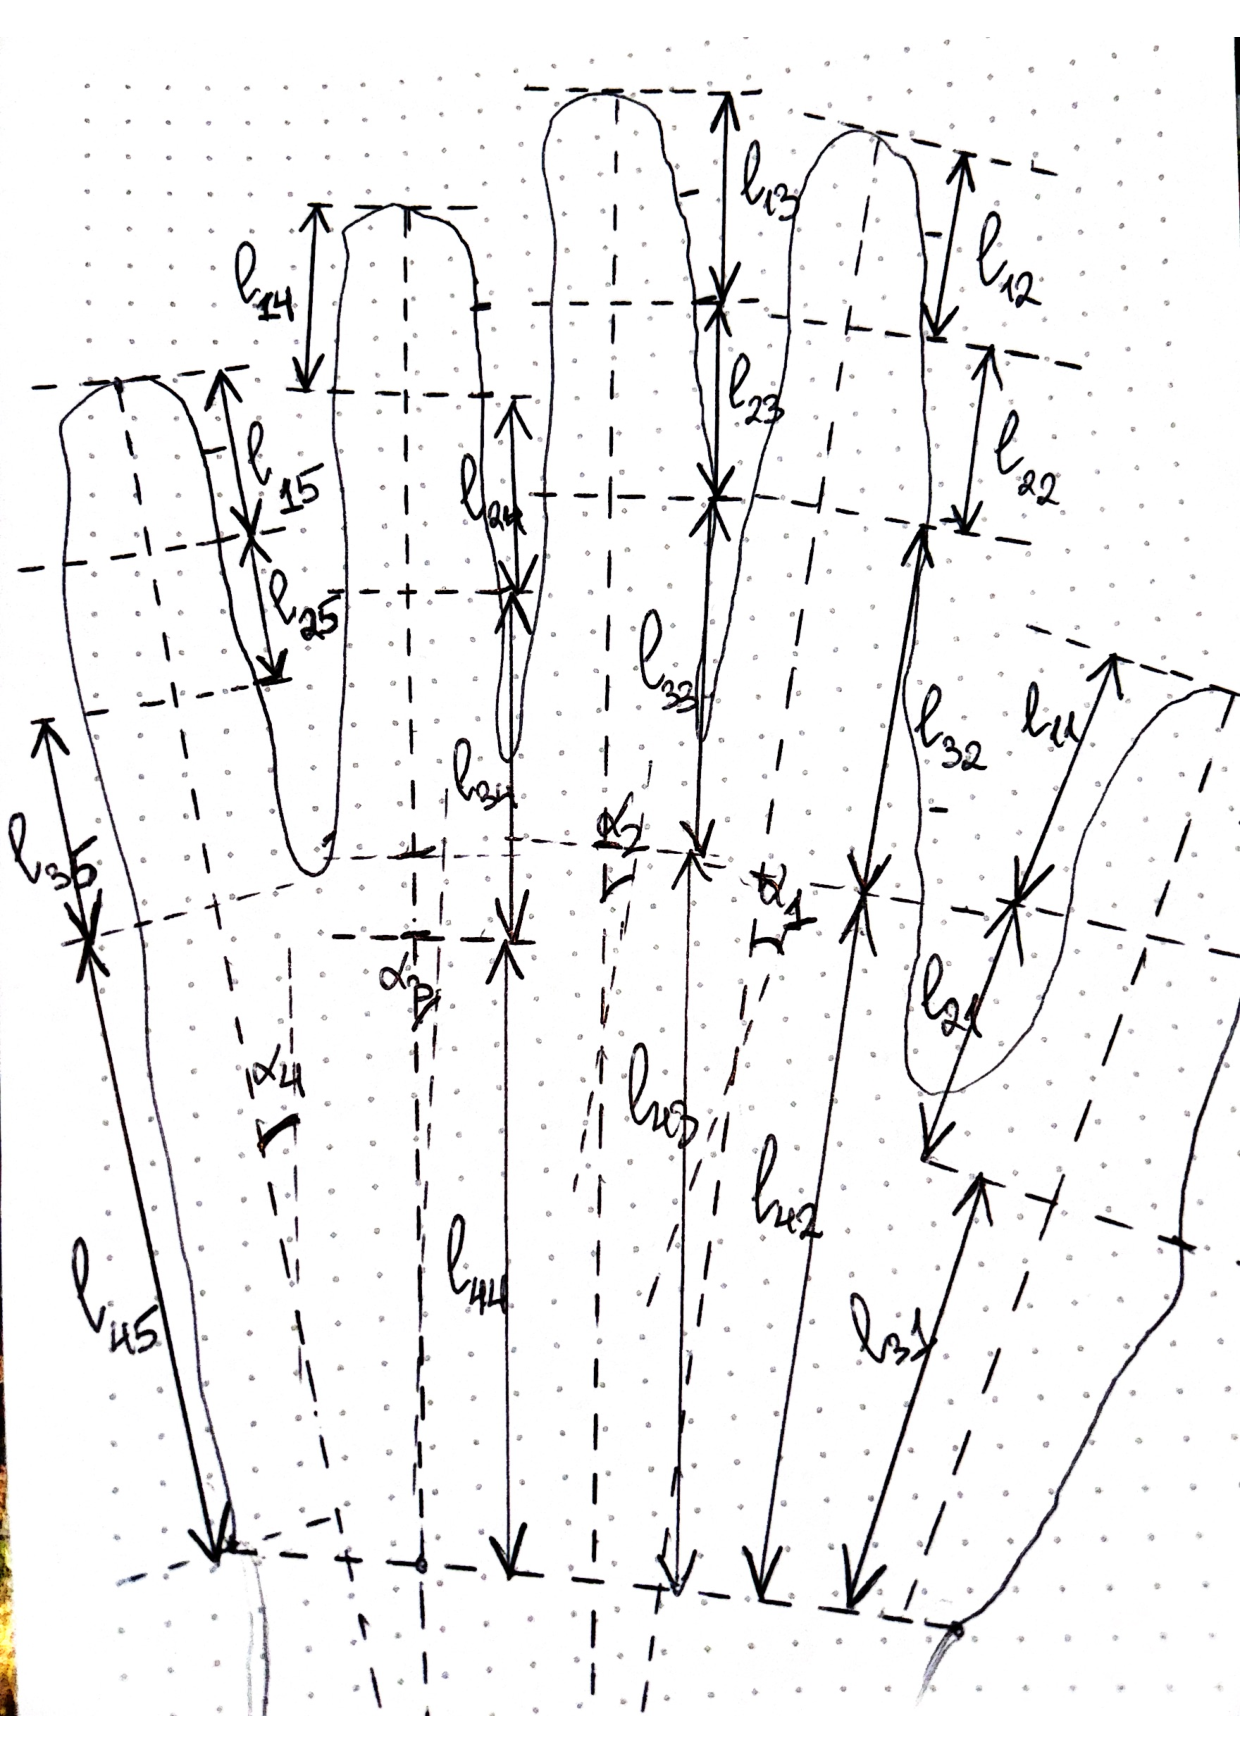
\includegraphics[width=0.8\textwidth]{images/left_rest.pdf}
    \caption{Ліва рука в спокійному стані.}
\end{figure}

\begin{figure}[H]
    \centering
    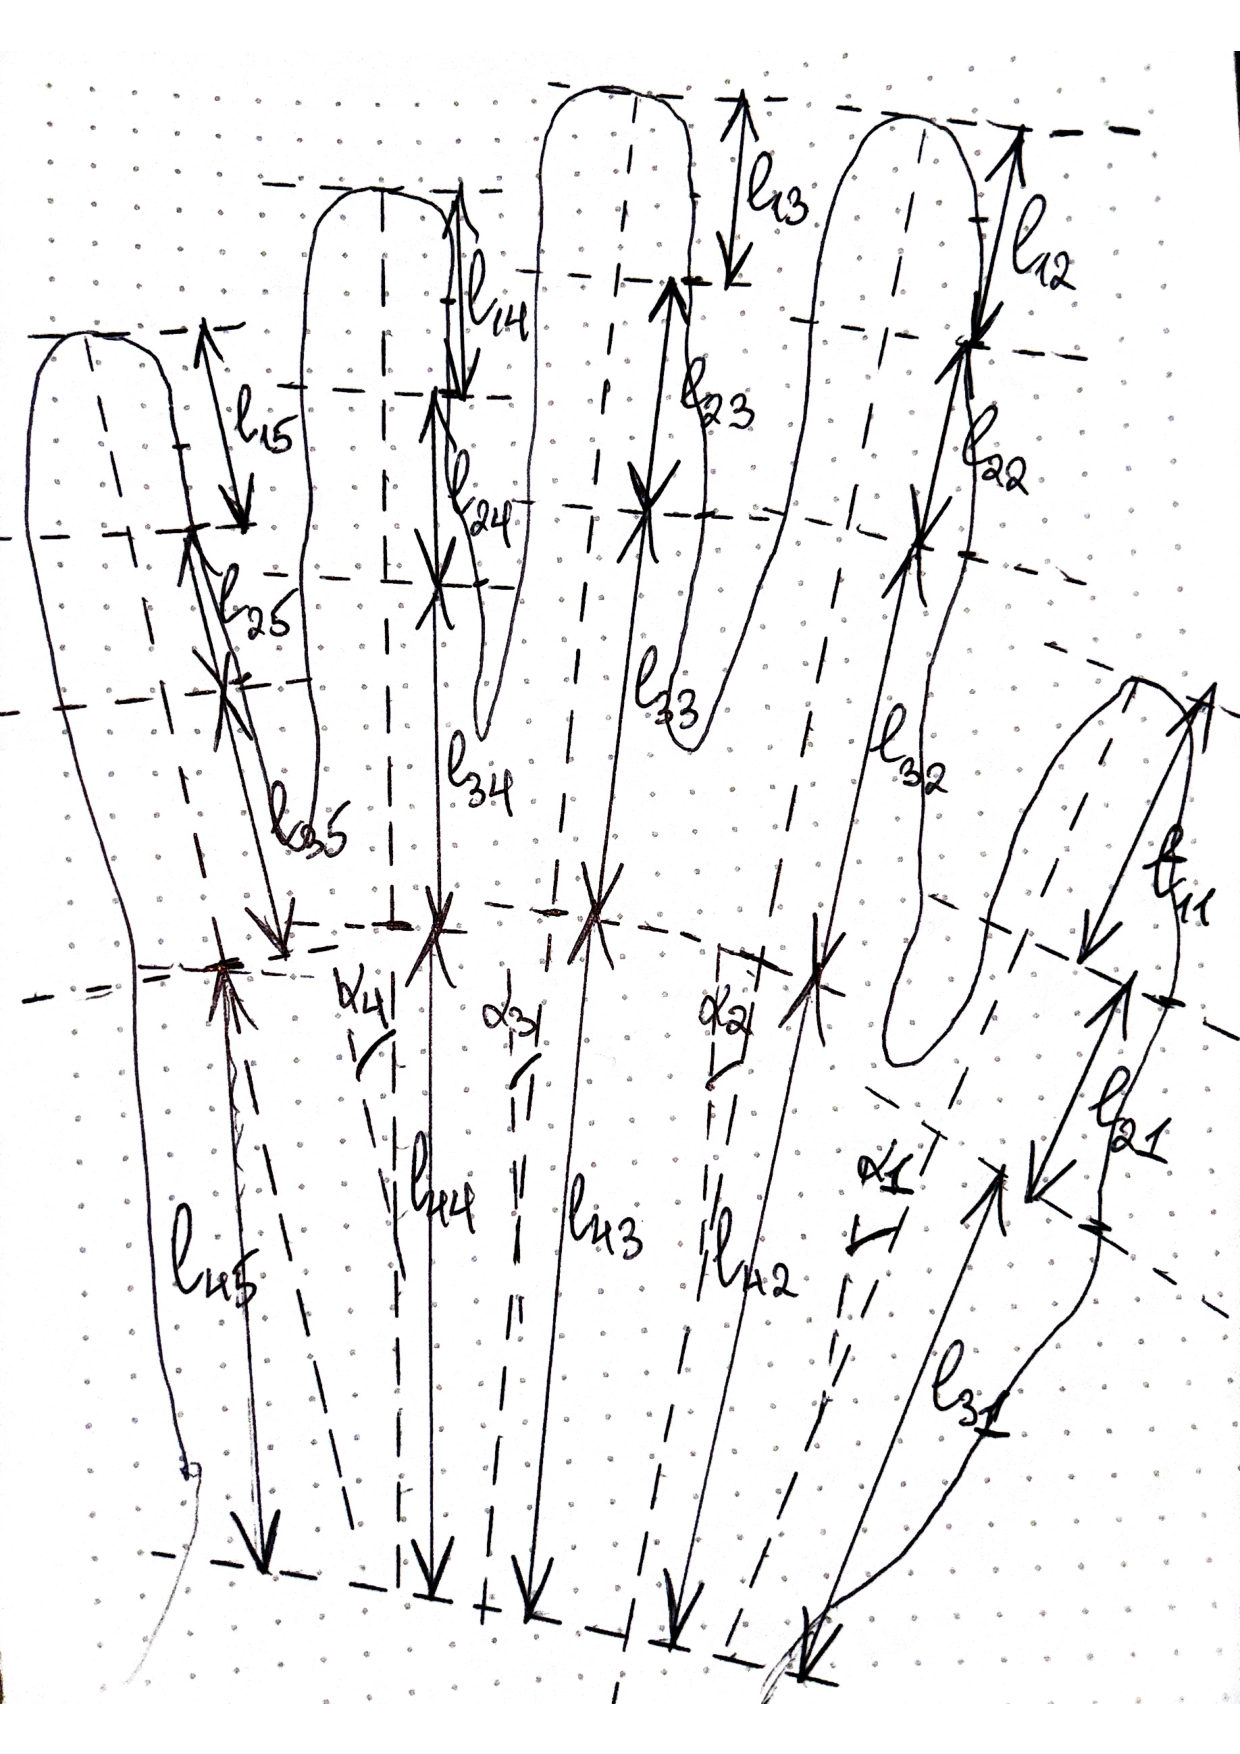
\includegraphics[width=0.8\textwidth]{images/left_stressed.pdf}
    \caption{Ліва рука в напруженому стані.}
\end{figure}

\begin{figure}[H]
    \centering
    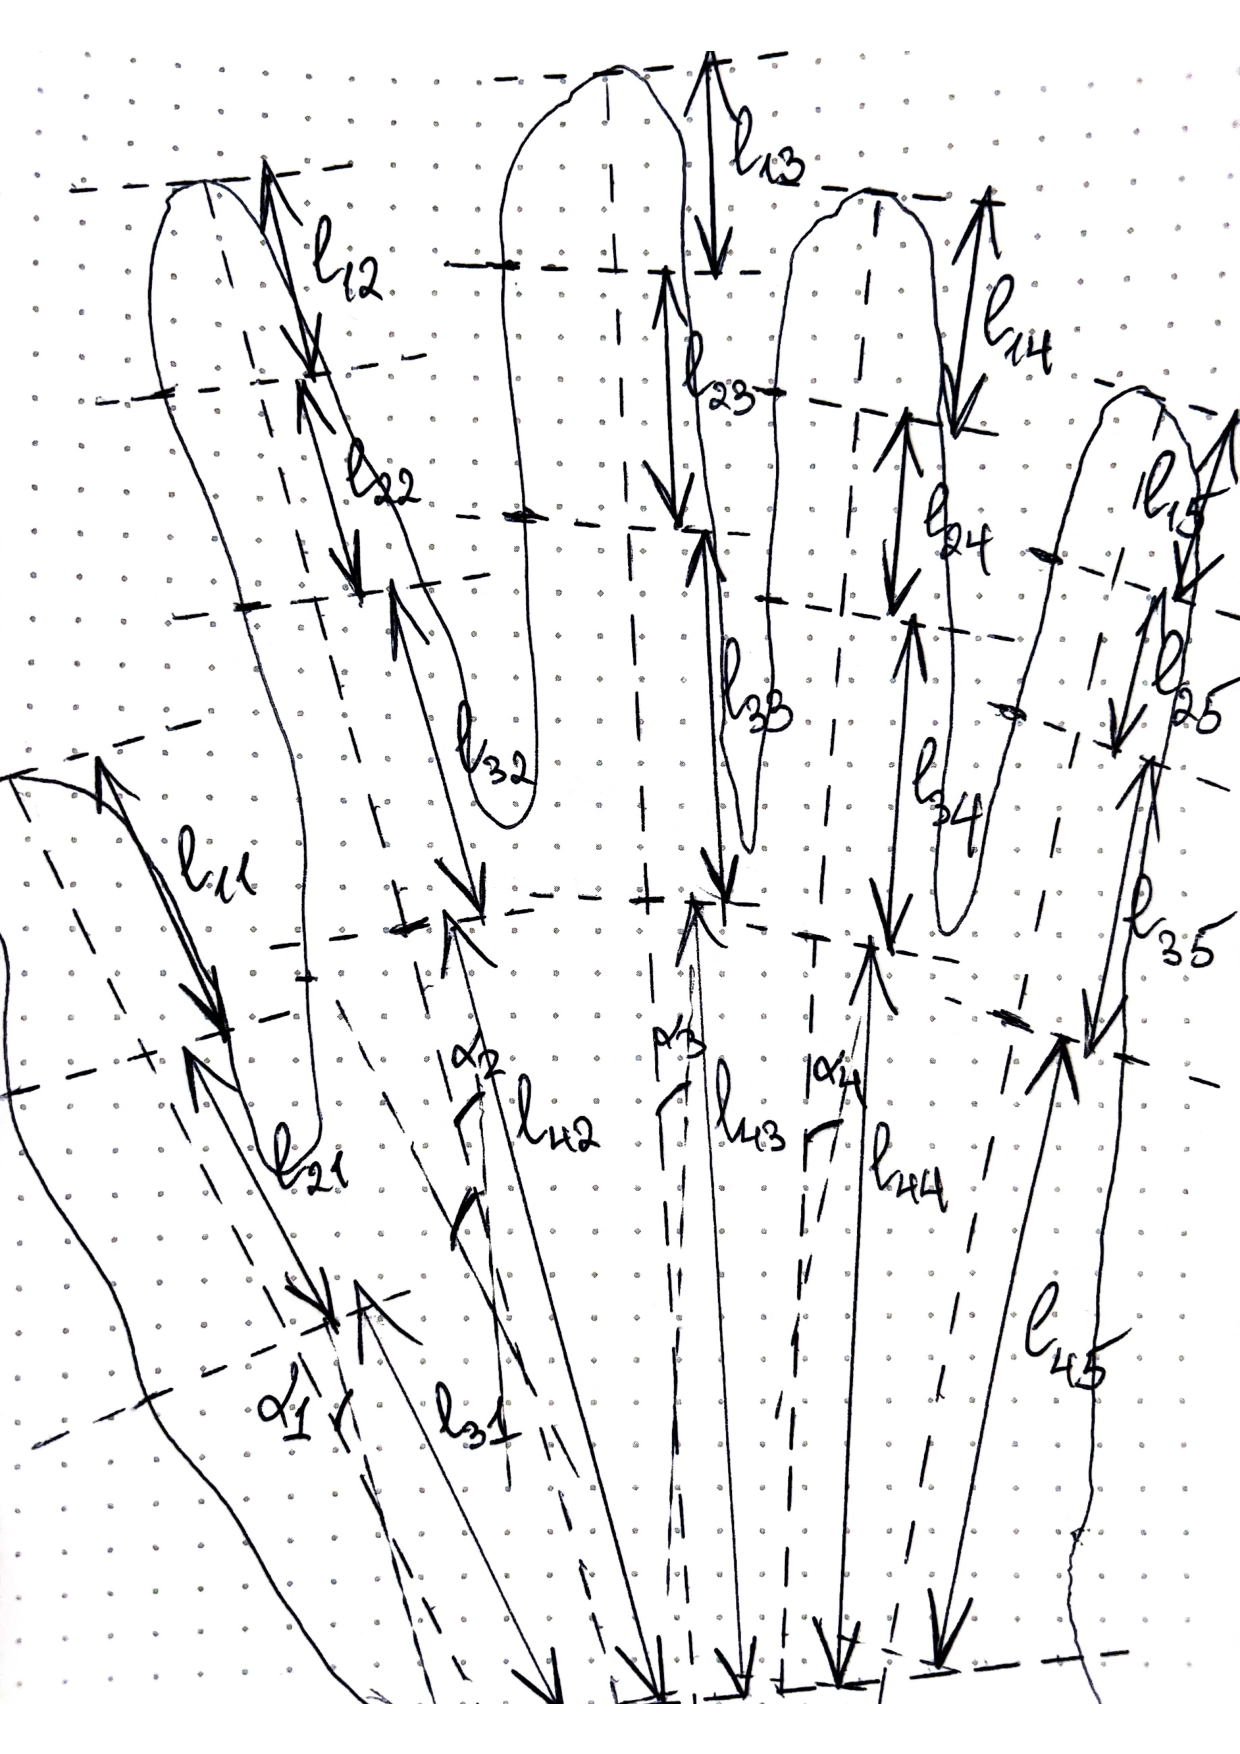
\includegraphics[width=0.8\textwidth]{images/right_rest.pdf}
    \caption{Права рука в спокійному стані.}
\end{figure}

\begin{figure}[H]
    \centering
    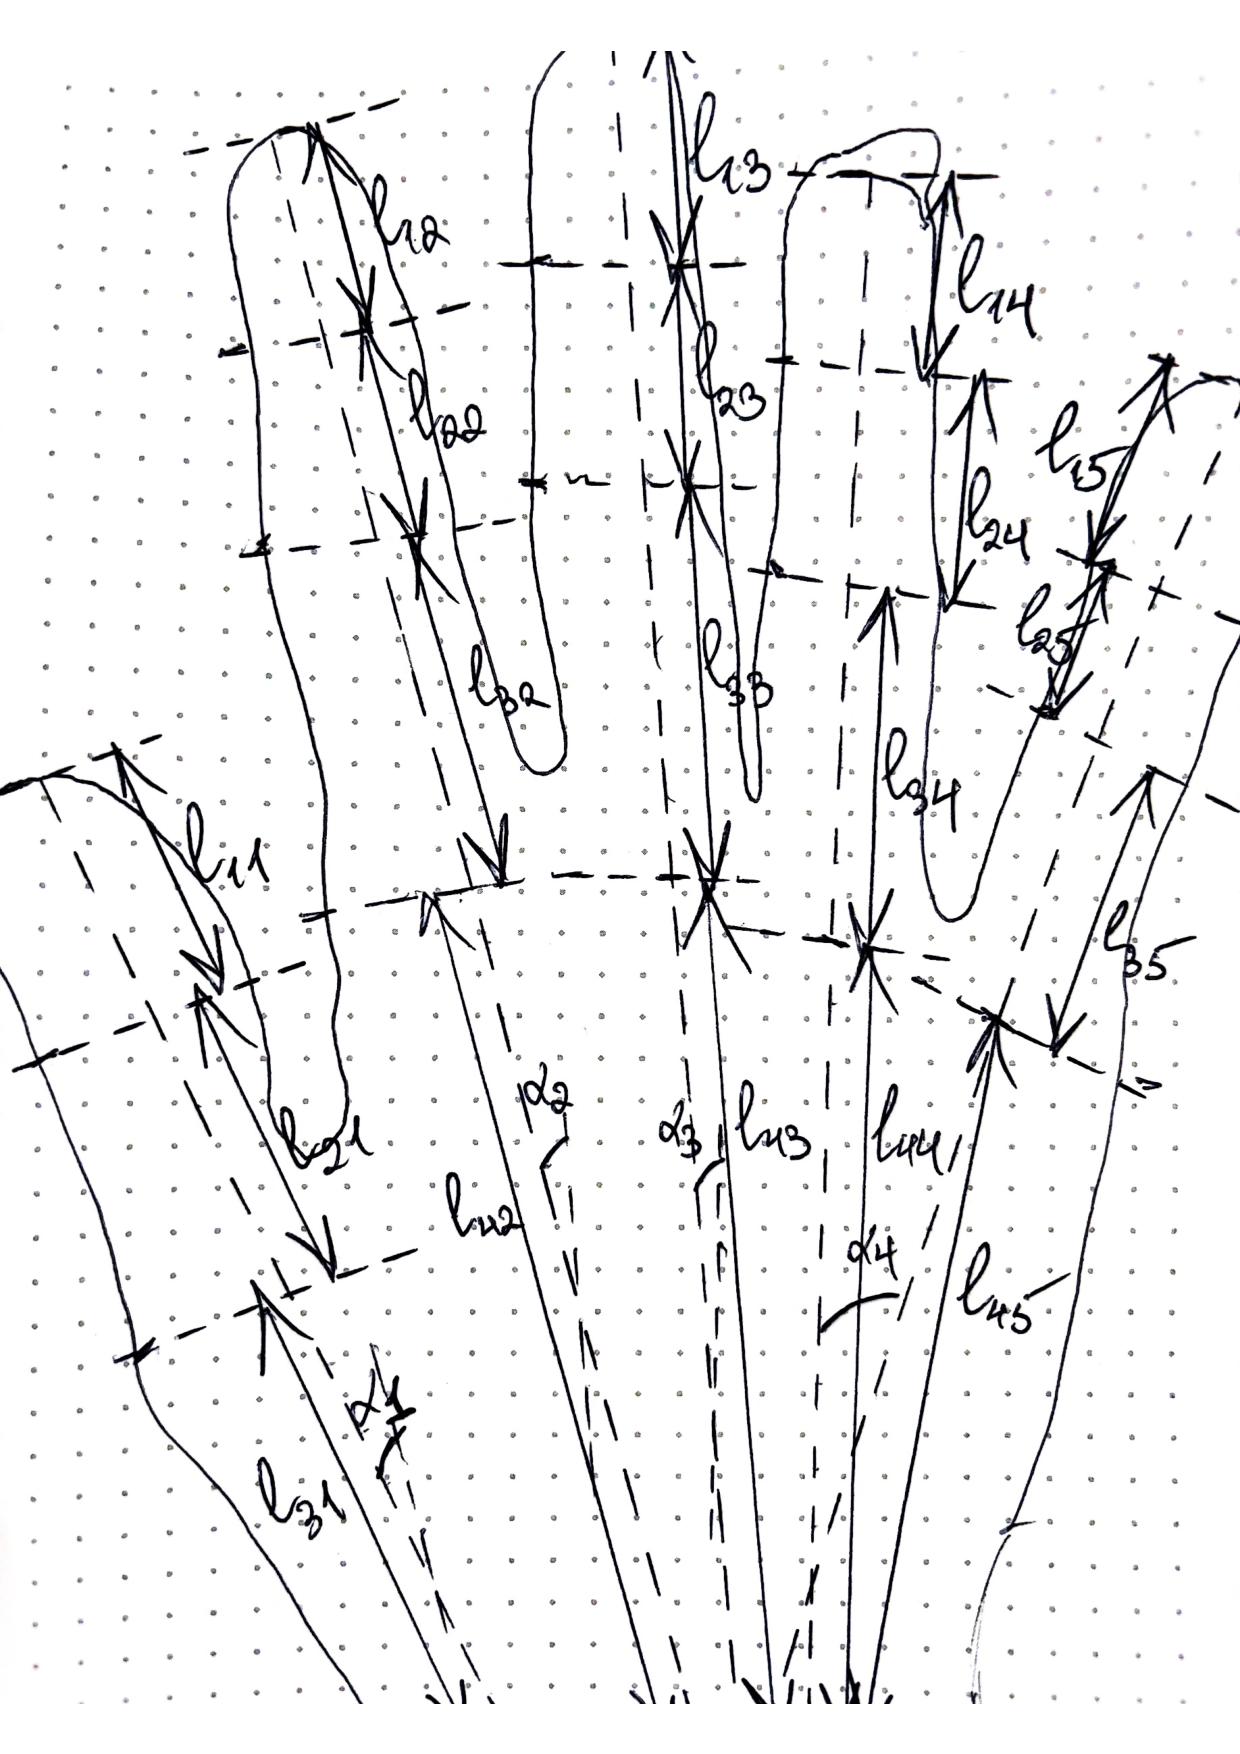
\includegraphics[width=0.8\textwidth]{images/right_stressed.pdf}
    \caption{Права рука в напруженому стані.}
\end{figure}

\end{document}